\chapter{Ergänzungen zur Laufzeitanalyse von Parsivald}
\label{appendix_runtime}

\section{Einfluss der Ereignis-Laufzeit auf die effiziente Raumgröße}

Die Ereignis-Laufzeit $T_\text{E}$ hat einen ähnlichen Einfluss auf $w_\text{eff}$ wie die MD-Laufzeit $T_\text{MD}$, doch ergibt sich eine inverse Proportionalität $w_\text{eff} \sim T_\text{E}^{-1}$, wie in Abbildung~\ref{fig:weffeventtime} zu erkennen ist.
Dieser Zusammenhang ergibt sich aus dem höheren Ereignisdurchsatz $R_\text{E}$ des Hauptprozesses, mit dem $p_\text{max,2}$ steigt.
Somit verschiebt sich die Grenze $w_\text{eff}$, für die $p_\text{max,1} = p_\text{max,2}$ gilt, weiter nach oben, wodurch größere Räume effizient betrachtet werden können.

\begin{figure}[p]

  \captionsetup[subfigure]{singlelinecheck=false}
  \def\subfigwidth{7cm}
  \begin{subfigure}[t]{\subfigwidth}
    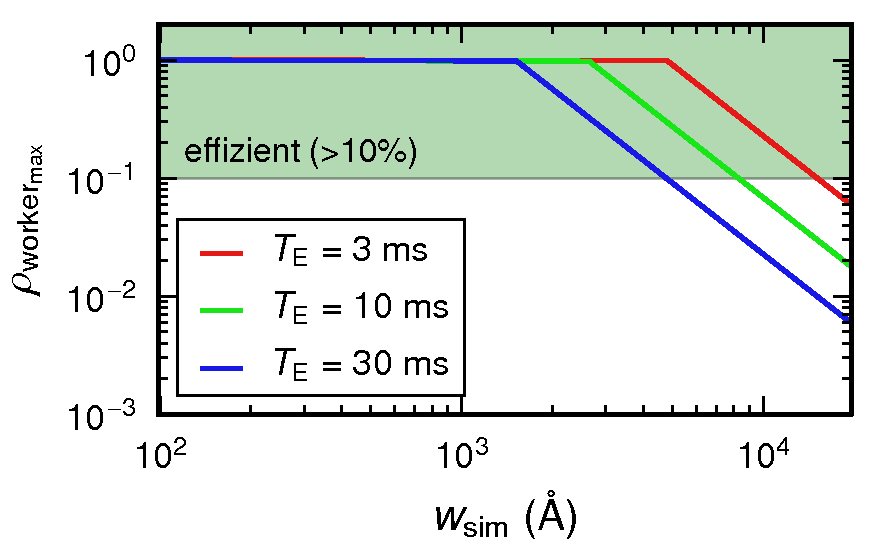
\includegraphics[width=\textwidth]{densitybykmctime}
  \end{subfigure}
  \hfill
  \begin{subfigure}[t]{\subfigwidth}
    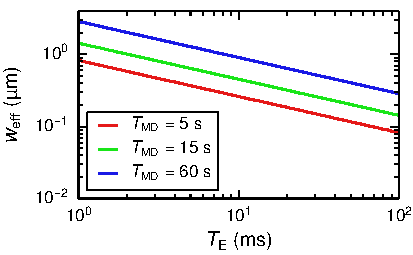
\includegraphics[width=\textwidth]{maxsizebykmctime}
  \end{subfigure}

  \caption{Einfluss der Ereignis-Laufzeit $T_\text{E}$ auf die effiziente Simulationsgröße $w_\text{eff}$}
  \label{fig:weffeventtime}

\end{figure}

\section{Zusätzliche Einflüsse auf das Maximum der Prozesse \texorpdfstring{$p_\text{max}$}{pmax}}

Zusätzlich zur Ereignis- und MD-Laufzeit wird $p_\text{max}$ über die Größe der MD-Boxen $w_\text{MD}$ und die maximale Workerdichte $\rho_\text{worker,max}$ während der Simulation beeinflusst (Abbildung~\ref{fig:pmaxother}).
$\rho_\text{worker}$ ist dabei von der Verteilung der Adsorptionsorte auf der Oberfläche abhängig und hat für gleichverteilte Simulationen von Gold-PVD Werte zwischen \SI{10}{\percent} und \SI{20}{\percent} angenommen.
Für stärker lokalisierte Adsorptionen sind aufgrund der überlappenden MD-Boxen und der daraus resultierenden Abhängigkeit der Ereignisse geringere Werte für $\rho_\text{worker}$ zu erwarten.
Es gilt $w_\text{eff} \sim \rho_\text{worker,max}^{-1}$

Die Erhöhung von $w_\text{MD}$ hat umfangreichere Einflüsse und verursacht eine Verringerung von $\rho_\text{max}$ aufgrund der Größe der Box, sowie eine Erhöhung von $T_\text{MD}$ und $T_\text{E}$ aufgrund der größeren Zahl an Atomen in der Box, was insgesamt zu einer Erhöhung von $w_\text{eff}$ führt.
Somit wird $p_\text{max}$ für $w_\text{sim} < w_\text{eff}$ verringert und für $w_\text{sim} > w_\text{eff}$ erhöht.
Da mit der Vergrößerung der MD-Boxen auch die gesamte Laufzeit nahezu proportional skaliert (Abbildung~\ref{fig:tpother}), wird $w_\text{MD}$ meistens minimal gewählt.

\section{Abschätzung der maximalen Workerdichte per Random Sequential Adsorption}
Bei Random Sequential Adsorption (RSA) werden beliebige Objekte nichtüberlappend an zufälligen Positionen auf einer Oberfläche verteilt, bis kein weiteres Objekt platziert werden kann.
Die Verteilung der Worker auf der Oberfläche geschieht auf eine ähnliche Weise, sodass als Grenzwert der Workerdichte \SI{56.2}{\percent}\cite{brosilow_random_1991} angegeben werden kann.
Da überlappende MD-Boxen in Parsivald nicht komplett abgelehnt werden, sondern ihre Berechnung nur bis zum Abschluss des überdeckten Ereignisses zurück gestellt wird und sich so ein kompletter Abhängigkeitsbaum bildet\cite{lorenz_entwicklung_2012}, liegt die Workerdichte typischerweise unterhalb dieses Wertes\todo{maximale Workerdichte plotten?}.

\begin{figure}[p]

  \captionsetup[subfigure]{singlelinecheck=false}
  \def\subfigwidth{7cm}
  \begin{subfigure}[t]{\subfigwidth}
    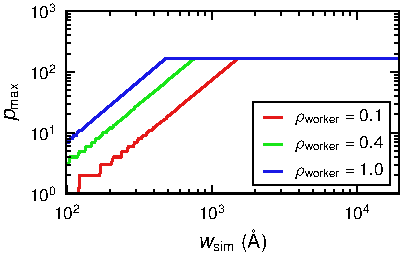
\includegraphics[width=\textwidth]{workersbydensity}
  \end{subfigure}
  \hfill
  \begin{subfigure}[t]{\subfigwidth}
    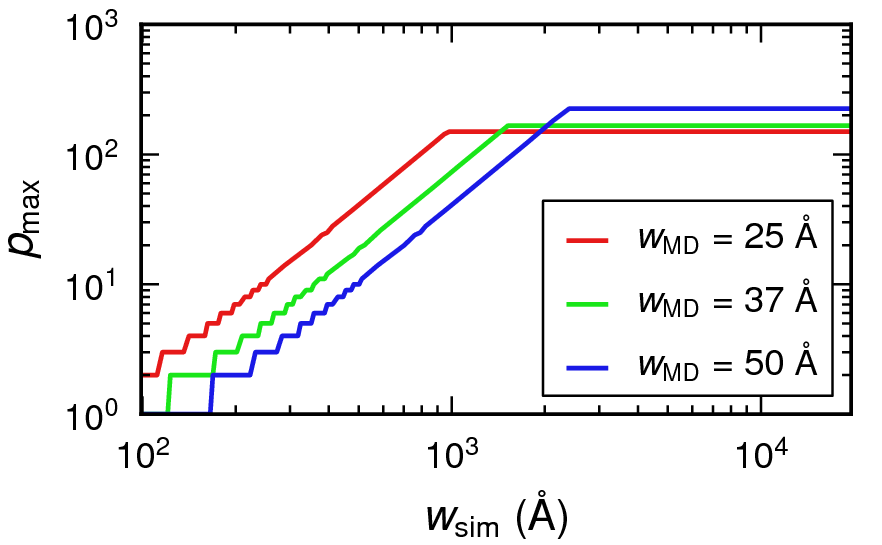
\includegraphics[width=\textwidth]{workersbymdsize}
  \end{subfigure}

  \caption{Einfluss von $\rho_\text{worker}$ und $w_\text{MD}$ auf die Laufzeit $p_\text{max}$}
  \label{fig:pmaxother}

\end{figure}

\begin{figure}[p]

  \captionsetup[subfigure]{singlelinecheck=false}
  \def\subfigwidth{7cm}
  \begin{subfigure}[t]{\subfigwidth}
    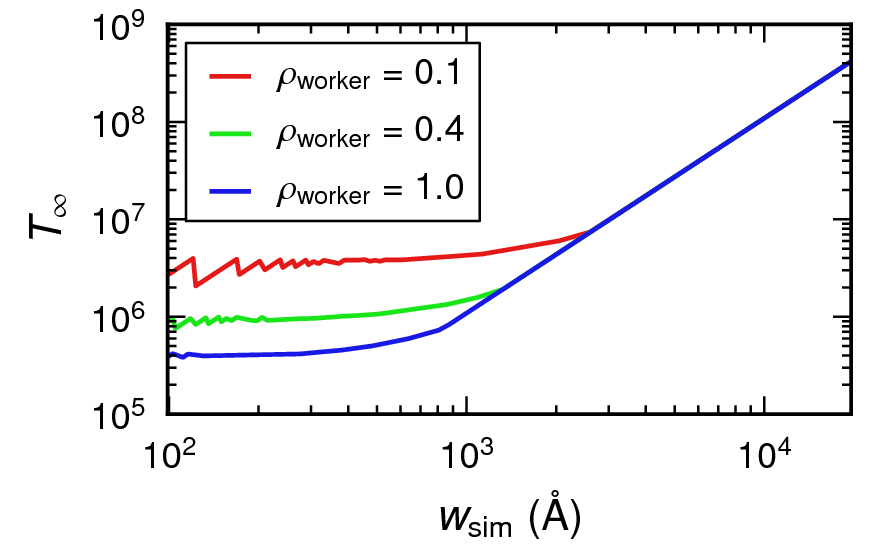
\includegraphics[width=\textwidth]{runtimebydensity}
  \end{subfigure}
  \hfill
  \begin{subfigure}[t]{\subfigwidth}
    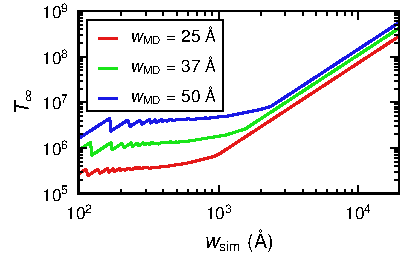
\includegraphics[width=\textwidth]{runtimebymdsize}
  \end{subfigure}

  \caption{Einfluss von $\rho_\text{worker}$ und $w_\text{MD}$ auf die Laufzeit $T_p$}
  \label{fig:tpother}

\end{figure}
